% Cartoon cross-section schematic of the Enceladus crack model (Figure 2).
% Standalone: compile with `tectonic schematic.tex` -> schematic.pdf, then
% 
\includegraphics{Figures/schematic.pdf} in main.tex.
\documentclass[border=3pt]{standalone}
\usepackage{tikz}
\usepackage{amsmath}
\usetikzlibrary{shadings,decorations.pathmorphing,decorations.markings,
                arrows.meta,positioning,calc,shapes.geometric,fadings}

% ---- palette ------------------------------------------------------------
\definecolor{spacetop}{RGB}{6,10,30}
\definecolor{spacebot}{RGB}{22,32,70}
\definecolor{icetop}{RGB}{205,228,242}
\definecolor{icebot}{RGB}{150,196,226}
\definecolor{water}{RGB}{42,116,196}
\definecolor{waterdk}{RGB}{20,74,146}
\definecolor{vapor}{RGB}{236,246,252}
\definecolor{walllayer}{RGB}{247,187,120}
\definecolor{sun}{RGB}{255,214,74}
\definecolor{heatred}{RGB}{214,64,48}
\definecolor{condgreen}{RGB}{31,140,110}

\newcommand{\region}[4]{% (x,y) number fillcolor
  \node[circle,fill=#4,text=white,inner sep=0pt,minimum size=6.5mm,
        font=\bfseries\small,draw=white,line width=0.4pt] at (#1,#2) {#3};}

\begin{document}
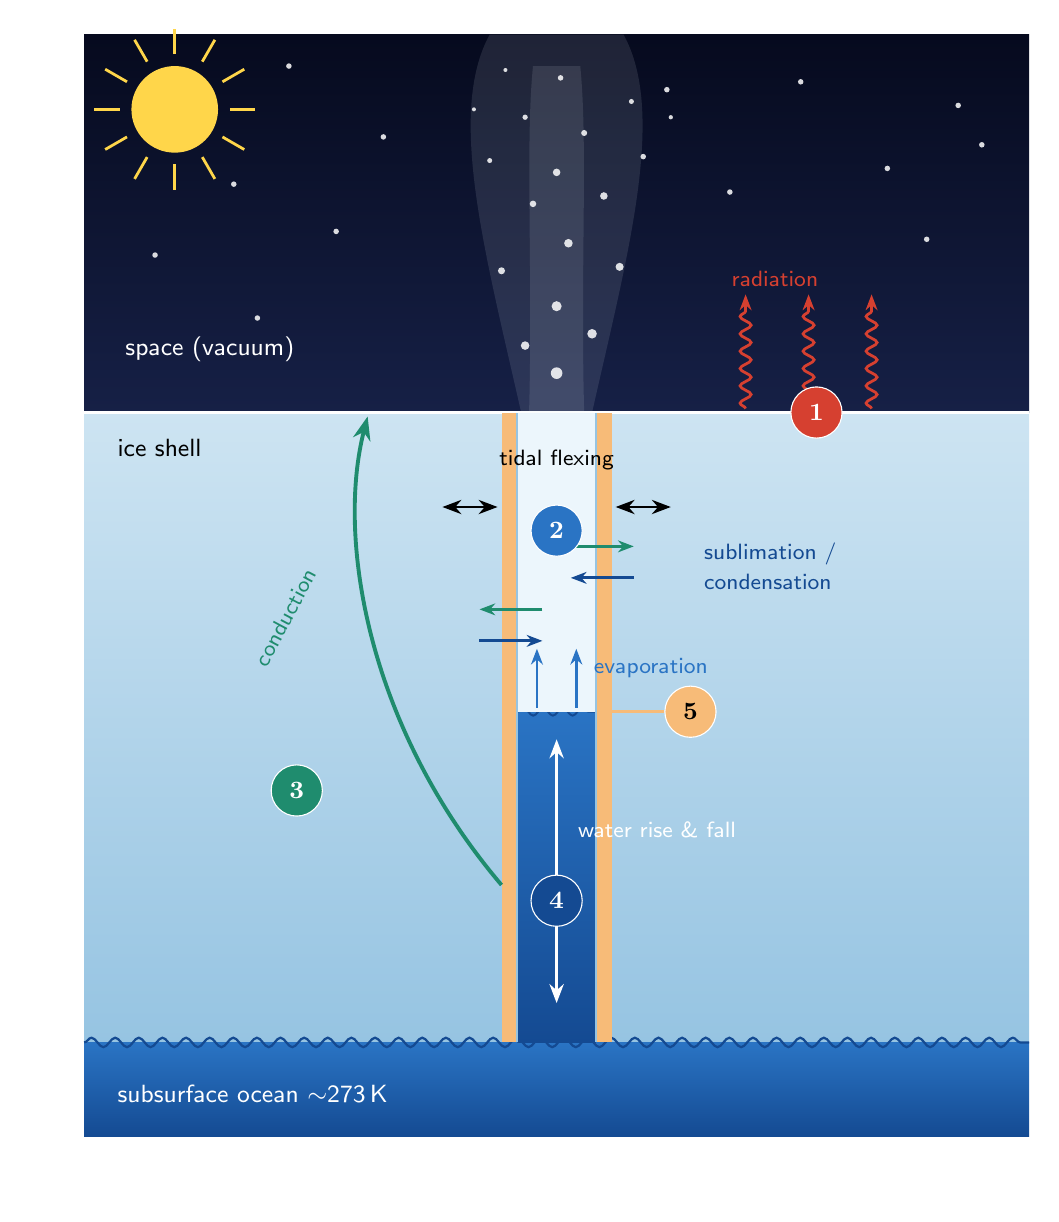
\begin{tikzpicture}[x=1cm,y=1cm]
  % canvas 0..12 wide, 0..14 tall; surface at y=9.2, ocean top at y=1.2
  \def\surf{9.2}\def\ocean{1.2}\def\xL{5.5}\def\xR{6.5}\def\wlev{5.4}

  % --- space -------------------------------------------------------------
  \shade[top color=spacetop,bottom color=spacebot]
        (0,\surf) rectangle (12,14);
  % stars (fixed positions)
  \foreach \sx/\sy in {0.7/13.2, 1.9/12.1, 2.6/13.6, 3.8/12.7, 9.1/13.4,
        10.2/12.3, 11.1/13.1, 8.2/12.0, 10.7/11.4, 0.9/11.2, 3.2/11.5,
        11.4/12.6, 7.4/13.3, 2.2/10.4}
     \fill[white,opacity=0.85] (\sx,\sy) circle (0.035);
  % sun
  \begin{scope}
    \fill[sun] (1.15,13.05) circle (0.55);
    \foreach \a in {0,30,...,330}
      \draw[sun,line width=1pt] (\a:0.7)++(1.15,13.05)
            -- ($(1.15,13.05)+(\a:1.02)$);
  \end{scope}

  % --- ice shell ---------------------------------------------------------
  \shade[top color=icetop,bottom color=icebot] (0,\ocean) rectangle (12,\surf);
  % surface line
  \draw[white,line width=1.1pt] (0,\surf) -- (12,\surf);

  % --- ocean at base -----------------------------------------------------
  \shade[top color=water,bottom color=waterdk] (0,0) rectangle (12,\ocean);
  \draw[waterdk,line width=0.8pt,decorate,
        decoration={snake,amplitude=0.6mm,segment length=3mm}]
        (0,\ocean) -- (12,\ocean);

  % --- wall thermal layer (region 5): thin bands lining the crack --------
  \fill[walllayer] (\xL-0.20,\ocean) rectangle (\xL,\surf);
  \fill[walllayer] (\xR,\ocean) rectangle (\xR+0.20,\surf);

  % --- liquid column in the crack ---------------------------------------
  \shade[top color=water,bottom color=waterdk]
        (\xL,\ocean) rectangle (\xR,\wlev);
  \draw[waterdk,line width=0.7pt,decorate,
        decoration={snake,amplitude=0.5mm,segment length=2.5mm}]
        (\xL,\wlev) -- (\xR,\wlev);
  % --- gas column in the crack ------------------------------------------
  \fill[vapor] (\xL,\wlev) rectangle (\xR,\surf);
  % crack walls
  \draw[icebot,line width=0.6pt] (\xL,\ocean) -- (\xL,\surf);
  \draw[icebot,line width=0.6pt] (\xR,\ocean) -- (\xR,\surf);

  % --- plume erupting into space ----------------------------------------
  \begin{scope}
    % soft vapor envelope (teardrop), widening upward
    \fill[vapor,opacity=0.11]
        (\xL+0.05,\surf) .. controls (5.1,11.2) and (4.6,13.0) .. (5.15,14)
        -- (6.85,14) .. controls (7.4,13.0) and (6.9,11.2) .. (\xR-0.05,\surf)
        -- cycle;
    \fill[vapor,opacity=0.11]
        (\xL+0.15,\surf) .. controls (5.7,11.0) and (5.6,12.6) .. (5.7,13.6)
        -- (6.3,13.6) .. controls (6.4,12.6) and (6.3,11.0) .. (\xR-0.15,\surf)
        -- cycle;
    % grainy ice/vapor particles (x,y,size-factor)
    \foreach \px/\py/\ps in {6/9.7/2.3, 5.6/10.05/1.7, 6.45/10.2/1.9,
        6.0/10.55/2.0, 5.3/11.0/1.4, 6.8/11.05/1.6, 6.15/11.35/1.7,
        5.7/11.85/1.3, 6.6/11.95/1.5, 6.0/12.25/1.5, 5.15/12.4/1.0,
        7.1/12.45/1.1, 6.35/12.75/1.2, 5.6/12.95/1.05, 6.95/13.15/1.0,
        6.05/13.45/1.1, 4.95/13.05/0.8, 7.45/12.95/0.85, 5.35/13.55/0.8}
      \fill[white,opacity=0.85] (\px,\py) circle (0.032*\ps);
  \end{scope}

  % ======================= process arrows ================================
  % radiation to space (region 1)
  \foreach \rx in {8.4,9.2,10.0}
    \draw[heatred,line width=1pt,decorate,
          decoration={snake,amplitude=0.7mm,segment length=2.2mm,post length=1.6mm},
          -{Stealth[length=2mm]}] (\rx,\surf+0.05) -- (\rx,\surf+1.5);
  % conduction up through the ice (region 3)
  \draw[condgreen,line width=1.4pt,-{Stealth[length=3mm]}]
        (\xL-0.2,3.2) .. controls (3.6,5.2) and (3.2,7.6) .. (3.6,\surf-0.05);
  % sublimation / condensation exchange across the wall (region 2 <-> 5):
  % clear opposed pair -- vapour deposits onto the wall, wall sublimates back
  \draw[condgreen,line width=1pt,-{Stealth[length=2mm]}] (6.18,7.5) -- (6.98,7.5);
  \draw[waterdk,line width=1pt,-{Stealth[length=2mm]}]   (6.98,7.1) -- (6.18,7.1);
  \draw[condgreen,line width=1pt,-{Stealth[length=2mm]}] (5.82,6.7) -- (5.02,6.7);
  \draw[waterdk,line width=1pt,-{Stealth[length=2mm]}]   (5.02,6.3) -- (5.82,6.3);
  % evaporation at the gas-liquid interface
  \foreach \ex in {5.75,6.25}
    \draw[water,line width=1pt,-{Stealth[length=2mm]}] (\ex,\wlev+0.05) -- (\ex,\wlev+0.8);
  % water rise / fall in the liquid column
  \draw[white,line width=1.2pt,{Stealth[length=2.4mm]}-{Stealth[length=2.4mm]}]
        (6,\ocean+0.5) -- (6,\wlev-0.35);
  % tidal flexing of the walls
  \draw[black,line width=1pt,{Stealth[length=2.4mm]}-{Stealth[length=2.4mm]}]
        (4.55,8.0) -- (5.25,8.0);
  \draw[black,line width=1pt,{Stealth[length=2.4mm]}-{Stealth[length=2.4mm]}]
        (6.75,8.0) -- (7.45,8.0);

  % ======================= region labels =================================
  \region{9.3}{\surf}{1}{heatred}
  \region{6}{7.7}{2}{water}
  \region{2.7}{4.4}{3}{condgreen}
  \region{6}{3.0}{4}{waterdk}
  \node[circle,fill=walllayer,text=black,inner sep=0pt,minimum size=6.5mm,
        font=\bfseries\small,draw=white,line width=0.4pt] (r5) at (7.7,5.4) {5};
  \draw[walllayer,line width=1pt] (r5) -- (\xR+0.2,5.4);

  % ======================= text annotations ==============================
  \node[white,font=\sffamily\small,anchor=west] at (0.4,10.0) {space (vacuum)};
  \node[font=\sffamily\small,anchor=west] at (0.3,\surf-0.45) {ice shell};
  \node[white,font=\sffamily\small,anchor=west] at (0.3,0.55) {subsurface ocean $\sim$273\,K};
  \node[heatred,font=\sffamily\footnotesize,anchor=west] at (8.1,10.9) {radiation};
  \node[condgreen,font=\sffamily\footnotesize,rotate=62] at (2.55,6.6) {conduction};
  \node[waterdk,font=\sffamily\footnotesize,anchor=west] at (7.75,7.4)
        {sublimation /};
  \node[waterdk,font=\sffamily\footnotesize,anchor=west] at (7.75,7.05)
        {condensation};
  \node[font=\sffamily\footnotesize,anchor=south] at (6,8.35) {tidal flexing};
  \node[white,font=\sffamily\footnotesize,anchor=west] at (6.15,3.9)
        {water rise \& fall};
  \node[water,font=\sffamily\footnotesize,anchor=west] at (6.35,\wlev+0.55)
        {evaporation};
\end{tikzpicture}
\end{document}
